\clearpage{\pagestyle{empty}\cleardoublepage}
\chapter{Introduzione}

\section{Uno sguardo d'insieme}

Internet nacque verso la fine degli anni sessanta grazie ad un progetto militare statunitense. Allora si chiamava Arpanet ed era il prototipo di un nuovo sistema di difesa e di controspionaggio ideato nell'ambito della Guerra Fredda. All'atto della sua creazione, pochi importanti nodi del Nord America erano connessi tra loro e le linee di collegamento trasportavano semplici informazioni testuali a bassissime velocità.

Al giorno d'oggi, grazie al progresso della tecnologia, che ha introdotto nel mercato apparecchiature di rete e PC a prezzi modici, e della globalizzazione, che li ha portati in ogni angolo del pianeta, Internet è diventata la \emph{rete delle reti} e connette tra loro miliardi di utenti in tutto il mondo. Consentendo lo scambio a notevole velocità di contenuti anche piuttosto complessi come foto, filmati, videogame \dots , è il principale mezzo di comunicazione di massa. Tale aspetto è evidenziato anche in campo economico dal fatto che spesso le aziende vi si affacciano al fine di offrire nuovi ed innovativi servizi. Basti pensare all'ascesa nel panorama mondiale che stanno avendo Facebook, Twitter e YouTube, piuttosto che eBay.

Le risorse di rete non sono però illimitate e inoltre sono condivise da un numero sempre più elevato di utilizzatori, sia attraverso i computer che tramite l'uso dei cellulari di ultima generazione. Quindi è ovvio che bisogna sfruttare al meglio quelle disponibili. Di conseguenza, si ha la necessità di garantire agli utenti un certo livello di qualità di determinati servizi e allo stesso tempo di limitarne altri. Per esempio un negozio potrebbe volere che dai propri PC sia possibile comunicare celermente con il magazzino centrale, ed evitare che i propri dipendenti perdano tempo a guardare video su YouTube.

In risposta a questa esigenza, cominciarono ad essere elaborati dei programmi in grado di bloccare le comunicazioni indesiderate, i \emph{firewall}.

Queste applicazioni, fatte girare su macchine poste al confine tra una rete e l'altra, esaminano le informazioni in transito e prendono decisioni (se permettere o meno la comunicazione) basandosi sulla natura del traffico di dati.

L'evoluzione informatica, la facilità con cui ognuno può aggiungere funzionalità alla rete senza dover seguire un rigido processo di standardizzazione e la semplicità con cui si possono modificare (e falsificare) le informazioni, han però fatto sì che presto tali programmi restassero indietro rispetto al progresso di Internet, diventando quindi piuttosto obsoleti. Di fatto, data la grande possibilità di personalizzazione, non esistono più regole semplici ed immediate sulle quali basarsi.

C'è quindi bisogno di ripensare la struttura dei firewall per renderli più adatti alle reti attuali. Nasce così il progetto \emph{L7-Bridge}.

\section{Il progetto L7-Bridge}

Questo progetto si propone di rendere il firewall, componente ormai essenziale di ogni rete, in grado di ispezionare più approfonditamente il traffico al fine di riconoscere quale servizio (anche detto \emph{protocollo applicativo}) sta effettivamente utilizzando le risorse, ovviamente senza costituire esso stesso un elemento di rallentamento. Sarebbe infatti inutile avere un sistema che impieghi così tanto tempo per elaborare un pacchetto da rendere lentissima, o addirittura inutilizzabile, una rete, seppur all'avanguardia tecnologicamente e capace di trasportare grandissime quantità di dati.

In questo caso ci viene in aiuto la continua corsa dei produttori di processori nel realizzare CPU sempre più performanti, in grado di eseguire svariati miliardi di operazioni al secondo e quindi, in nostri termini, di processare moltissime informazioni.

Inoltre le astrazioni informatiche permettono, oltre a processare (virtualmente) in contemporanea più informazioni, anche dei meccanismi per catturarle dalla rete ad alta velocità per portarli direttamente al motore d'analisi del firewall, consentendo un'ulteriore accelerazione dell'elaborazione.

Insomma, le premesse ci sono tutte per rendere molto interessante muoversi in questa direzione, al fine di sviluppare un prodotto innovativo che potrà colmare il gap tra l'espansione dei servizi Internet e l'attuale concezione del firewall.

Gli amministratori di rete, per esempio, avranno a disposizione un programma flessibile, facilmente configurabile e aggiornabile, da poter utilizzare ogniqualvolta abbiano la necessità di filtrare certo traffico per garantire priorità a determinati protocolli applicativi e scoraggiare, o anche impedire, l'uso di altri.

Ovviamente tale obiettivo può essere raggiunto solo se la macchina ospitante l'applicazione è posta sul confine tra una rete e l'altra senza che vi sia possibilità di far passare il traffico attraverso altre postazioni da e verso l'esterno. Così facendo si ottiene un controllo totale sui flussi di comunicazione, garantendo una piena operatività dei filtri. Ne risulta quindi che l'ubicazione perfetta sia ad esempio in un PC con due schede di rete. Una sul lato della rete interna da sorvegliare, e l'altra sul lato del resto del mondo (come illustrato in figura \ref{ubifw}). Tale configurazione prende, in gergo di rete, il nome di \emph{bridge}.

Naturalmente è da qui, e dal proposito di riconoscere i protocolli applicativi (che sono concettualmente al livello 7 del modello ISO/OSI), che il progetto deve il suo nome.

\begin{figure}[!htbp] % H !htbp
\begin{center}
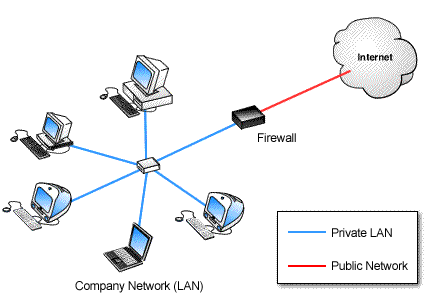
\includegraphics[scale=0.5]{img/ubicazione_fw.png}
\caption{Esempio di ubicazione del firewall}\label{ubifw}
\end{center}
\end{figure}

Lo sviluppo del codice è avvenuto in totale autonomia. Non sono comunque mancati l'appoggio e i suggerimenti preziosi del professore, che, data la sua esperienza nel campo del monitoraggio di reti ad alte prestazioni, hanno consentito un soddisfacente raggiungimento degli obiettivi preposti, con diverse possibilità di ampliamento futuro.

Anche grazie ad incontri appositi piuttosto costruttivi col professore per scambi di idee e pareri, sono state approfondite le conoscenze sui vari aspetti che riguardano la programmazione di rete, con particolare attenzione alle performance, aspetto centrale del progresso tecnologico.

%\clearpage

\section{Struttura della relazione di tirocinio}
{{\samepage
La relazione di tirocinio si articola su altri cinque capitoli, oltre a questo di carattere generale e introduttivo.
\begin{description}
\item[Capitolo 2] Dettaglio delle motivazioni, degli obiettivi e degli aspetti centrali del progetto.
\item[Capitolo 3] Implementazione scelta per risolvere il problema.
\item[Capitolo 4] Validazione e test a cui il sistema è stato sottoposto.
\item[Capitolo 5] Le altre soluzioni che ora il mercato mette a disposizione.
\item[Capitolo 6] Conclusioni a cui si è arrivati a seguito della realizzazione di questo progetto.
\end{description}
}}